\begin{frame}{Intuition}
  \begin{itemize}[<+>]
    \item Managed runtimes use garbage collectors to abstract away manual memory management
    \item These languages are simple to program in (e.g. Python, Haskell) without malloc
    \item Under the hood objects are placed in heap pages that are managed by the OS paging policy
  \end{itemize}

  \begin{block}{Why might we disagree with the OS policy?}
    \begin{itemize}[<+>]
      \item MLP: memory level parallelism
      \item OS has no idea what's on our pages. Could be a linked list (low MLP); could be a \texttt{std::array} (high MLP)
      \item Pointer chasing is expensive in low MLP objects. Latency is more affordable in high MLP objects
      \item Can we place our objects elsewhere? Where?
    \end{itemize}
  \end{block}
\end{frame}

\begin{frame}{Intuition}
  \begin{block}{Introduce: far memory}
    \begin{itemize}[<+>]
      \item Far memory is shared memory between devices that is cheaper and slower than RAM but faster than swap
      \item In HPC, we may accept the performance tradeoff if it means swapping fewer pages - overall still faster
      \item Thus, maybe some objects can live in near memory, others in far memory
      \item How can we automagically choose where heap objects live?
    \end{itemize}
  \end{block}
\end{frame}

\begin{frame}{Intuition}
  \begin{block}{mmap}
    \begin{itemize}[<+>]
      \item Map a file (e.g. a driver) into the address space, so we can write to it using vanilla pointers
      \item Some people hate mmap with a burning passion, namely those in our databases group
      \item That's for very understandable reasons!! DBMS developers are not friends with the OS which could destroy ACID properties
      \item We \textit{are} friends with the OS. We want to work with the paging policy to put our objects in reasonable places
      \item So we can just mmap a new region of memory to a far memory device, and that allows us to write objects to it as though it was normal RAM. Super easy to use!!
    \end{itemize}
  \end{block}
\end{frame}

\begin{frame}{The Project}
  \begin{block}{What are we doing?}
    \begin{itemize}[<+>]
      \item OCaml gc has minor and major heap pages. What that means is an implicit tier.
      \item Can we build on top of this tier? Some objects go near, others go far? Add a new tier to the existing layers?
      \item Can we trust that mmap is actually writing our bytes to the right device?
      \item What policy should we use to choose where to place objects?
      \item What if we want to move objects between near and far pages?
      \item What do we do?!?!
    \end{itemize}
  \end{block}
\end{frame}

\begin{frame}{Objects can be written to far memory with reasonable latency}
  \begin{center}
    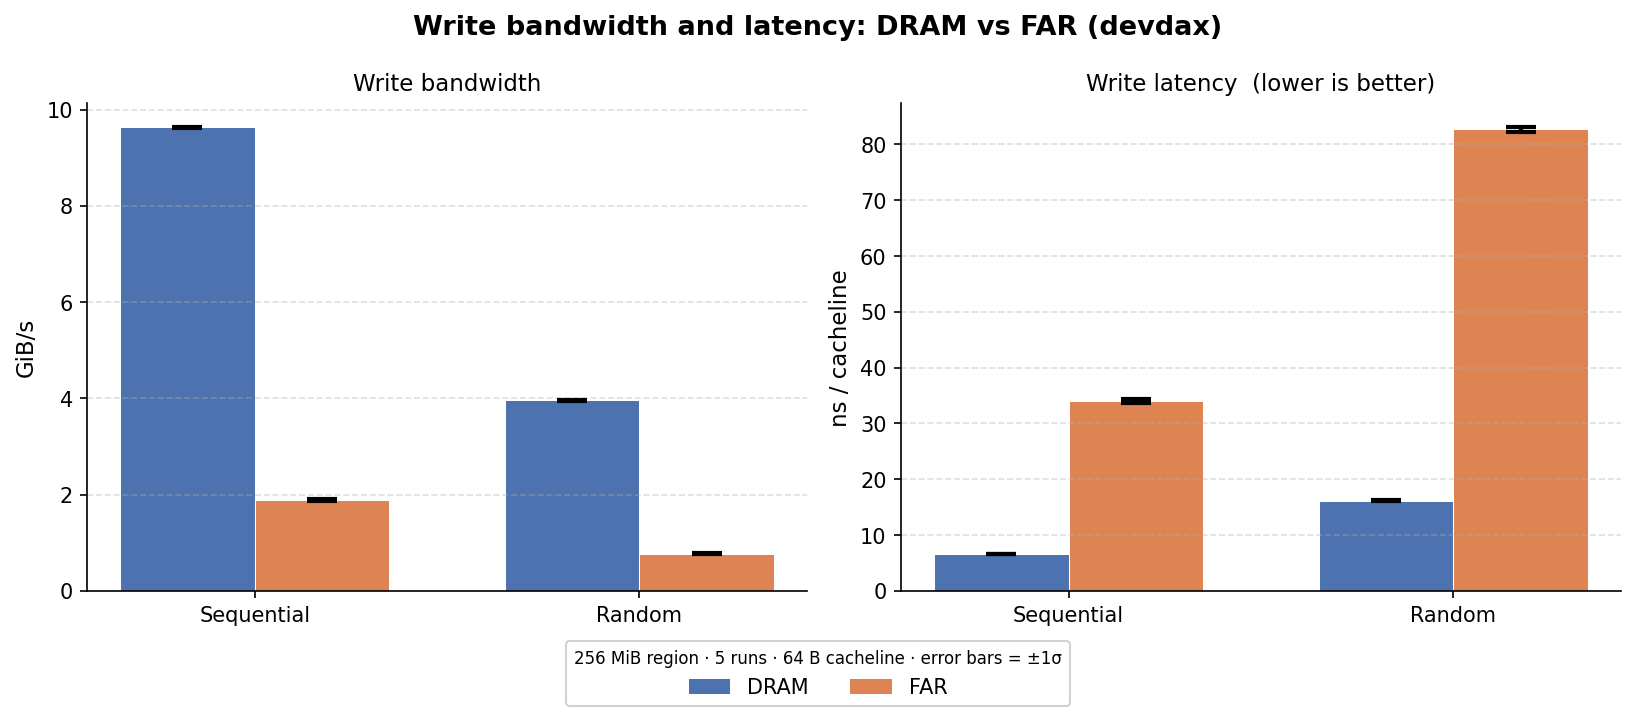
\includegraphics[width=0.8\linewidth]{figures/week4_write_bw.png}
  \end{center}
\end{frame}

\begin{frame}{Objects can be placed on near and far pages using mmap with consistent latencies}
  \begin{center}
    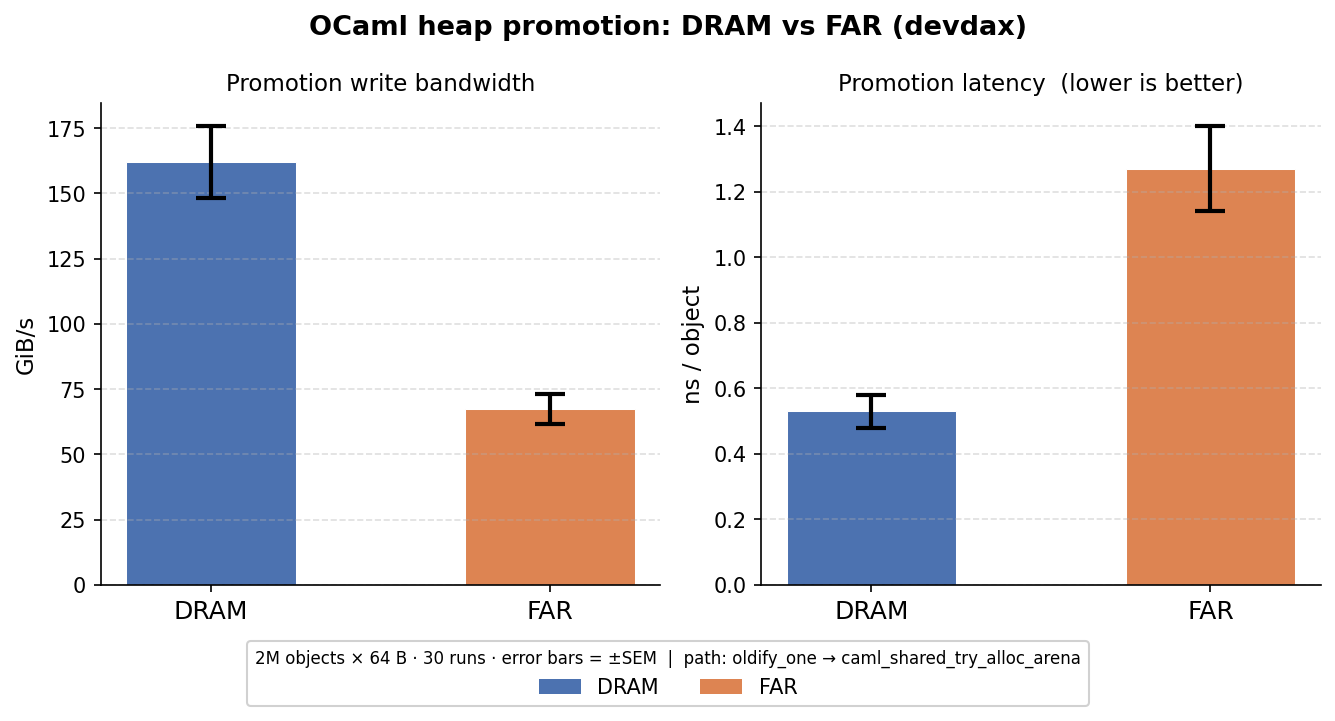
\includegraphics[width=0.8\linewidth]{figures/week4_heap_results.png}
  \end{center}
\end{frame}

\begin{frame}{Naive round robin policy is able to distribute objects across both near and far pages}
  \begin{center}
    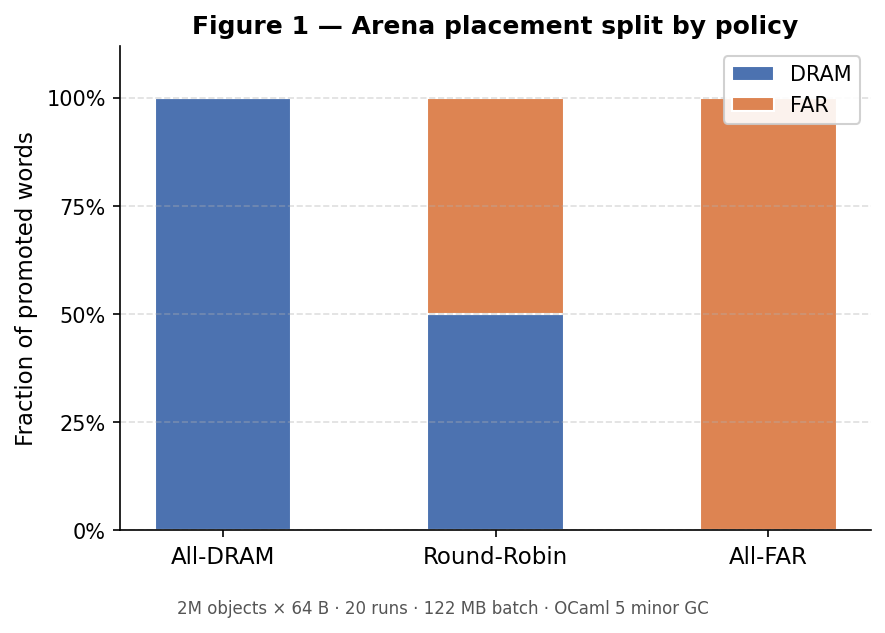
\includegraphics[width=0.8\linewidth]{figures/week5_results_fig1_split.png}
  \end{center}
\end{frame}

\begin{frame}{Some primitive MLP and hotness based metrics infrastructure engineered into OCaml runtime}
  \begin{center}
    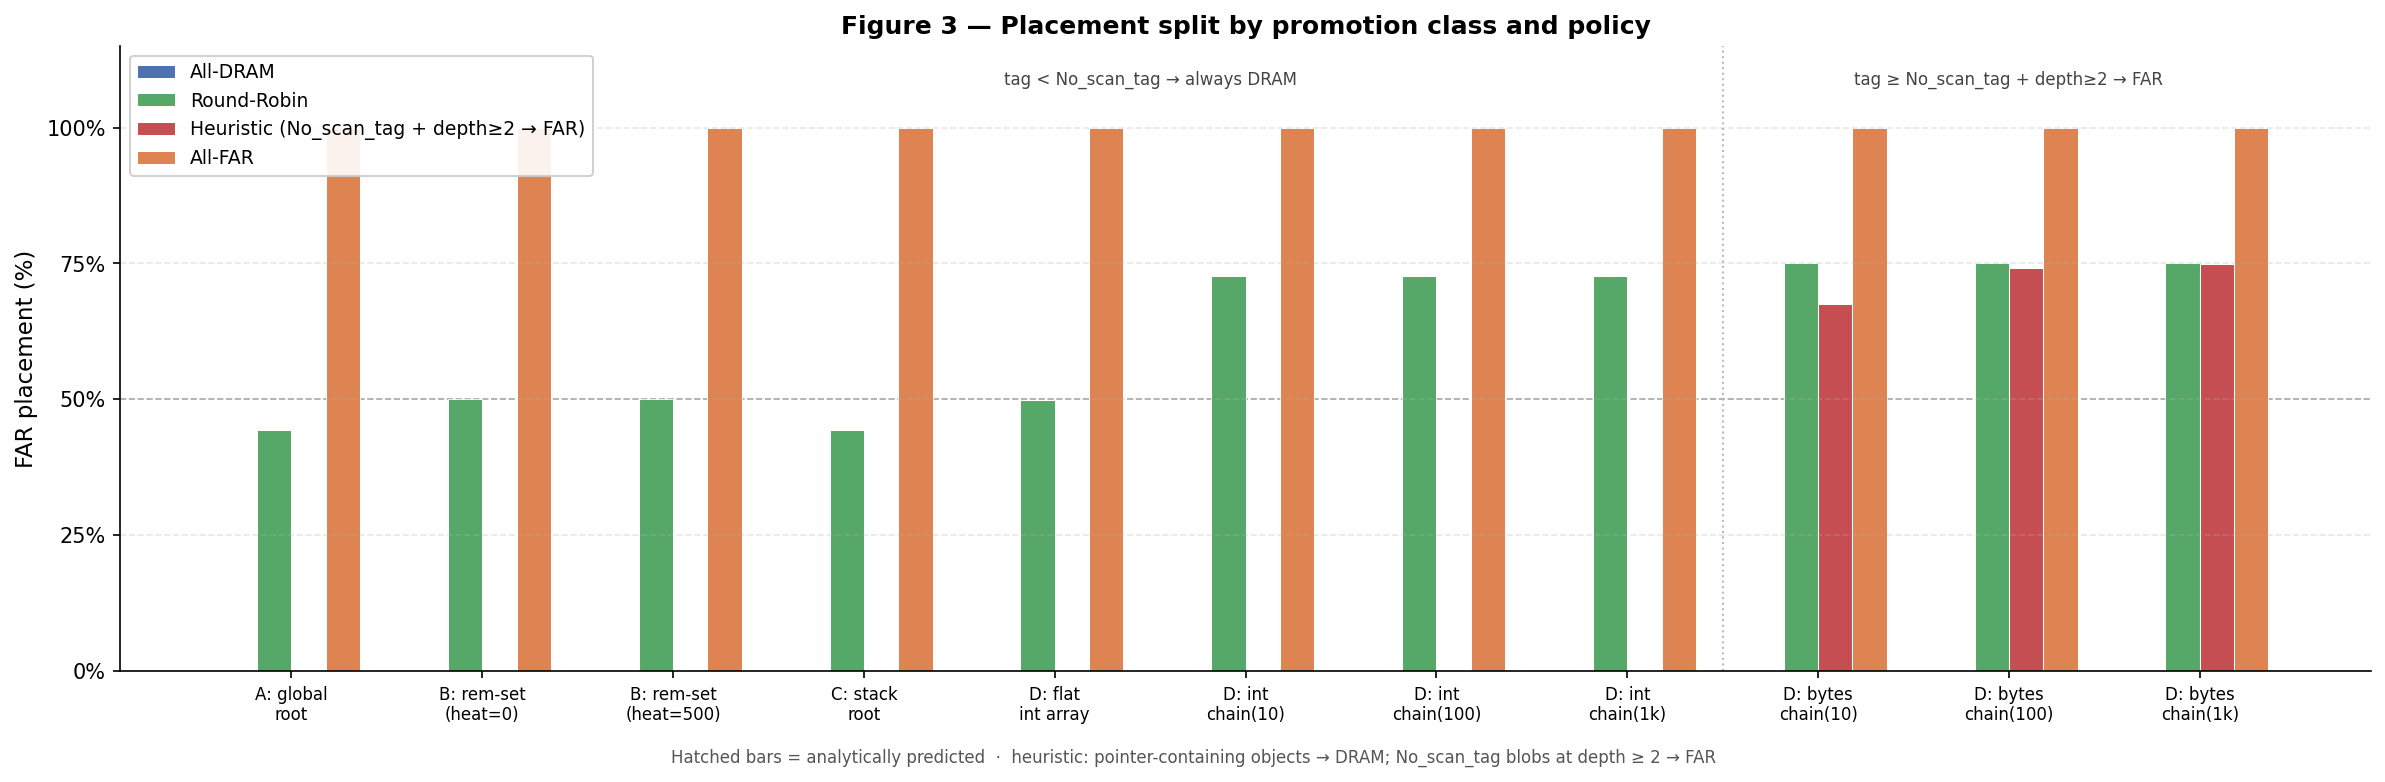
\includegraphics[width=0.8\linewidth]{figures/week6_classes_fig3_class_split.png}
  \end{center}
\end{frame}

\begin{frame}{Benchmarking}
  \begin{block}{Benchmark}
    \begin{itemize}[<+>]
      \item Use high memory-pressure programs. We want to trigger paging and gc collections.
      \item Have programs that dominantly used linked lists, some use parallel data structures, some use both
      \item Compare across policies: all DRAM, all far, round robin, and our heuristic that we are designing
    \end{itemize}
  \end{block}
\end{frame}

\begin{frame}{Benchmark does not work very well? This is the next week worth of work}
  \begin{center}
    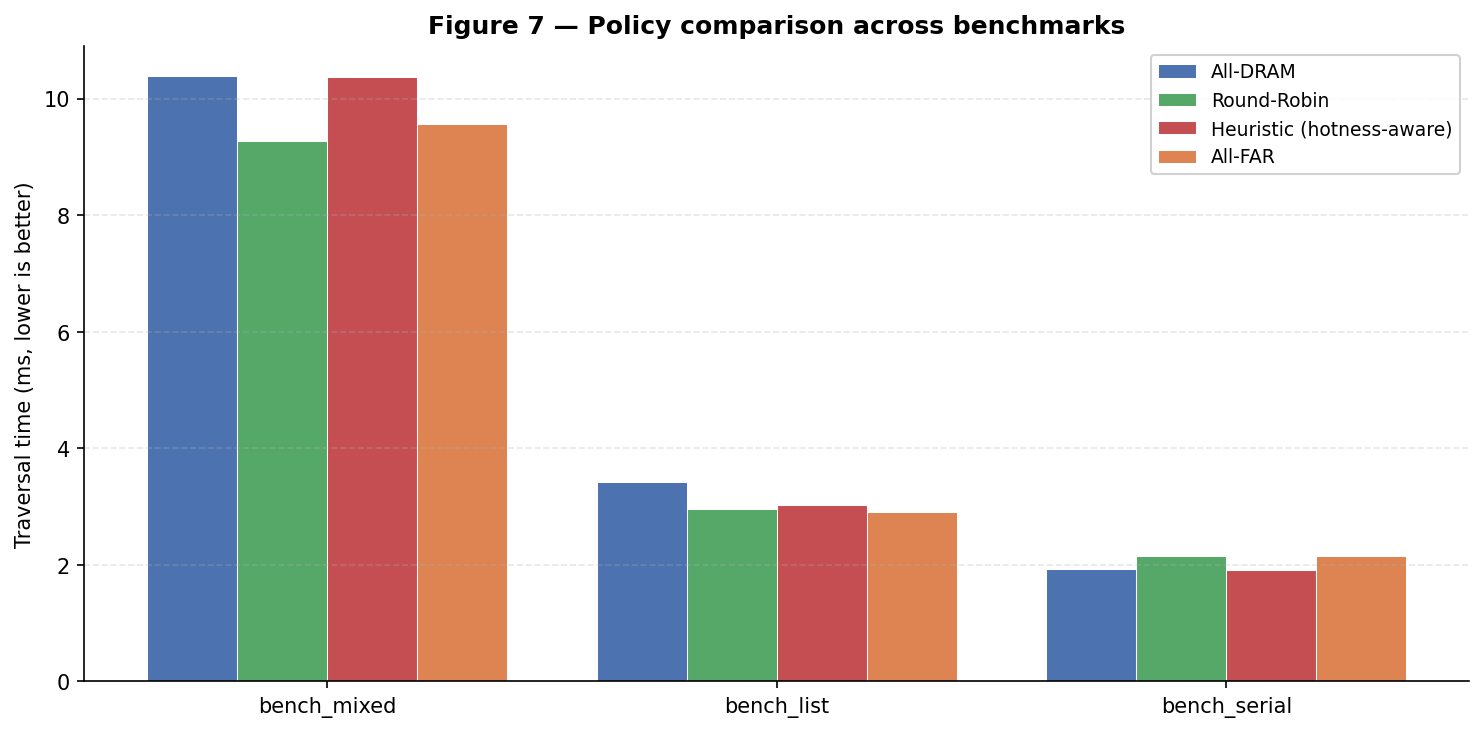
\includegraphics[width=0.8\linewidth]{figures/week7_fig7_policy_comparison.png}
  \end{center}
\end{frame}

\begin{frame}{Summary}
  \begin{block}{What are we doing?}
    \begin{itemize}[<+>]
      \item Not all objects are created equal
      \item Given limited RAM, we want all objects in DRAM to be sensitive enough to a slower memory latency that they justify the cost of some DRAM bytes
      \item Linked list, good example. Hash table with heap allocations, good example. Binary tree, good example. Pointer chasing creates slowness for every chase
      \item Array with independent elements, bad for DRAM, we might as well tank a single access latency if it means we can place another slower object in DRAM
      \item Essentially, we are engineering the opportunity cost of using DRAM into the OCaml runtime
    \end{itemize}
  \end{block}
\end{frame}
